\documentclass[12pt]{article}
\usepackage{geometry}                % See geometry.pdf to learn the layout options. There are lots.
\geometry{letterpaper}                   % ... or a4paper or a5paper or ... 
%\geometry{landscape}                % Activate for for rotated page geometry
\usepackage[parfill]{parskip}    % Activate to begin paragraphs with an empty line rather than an indent
\usepackage{daves,fancyhdr,natbib,graphicx,dcolumn,amsmath,lastpage,url}
\usepackage{amsmath,amssymb,epstopdf,longtable}
\usepackage{paralist} 
\DeclareGraphicsRule{.tif}{png}{.png}{`convert #1 `dirname #1`/`basename #1 .tif`.png}
\pagestyle{fancy}
\lhead{CE 3372 -- Water Systems Design}
\rhead{SPRING 2025}
\lfoot{EXERCISE 7}
\cfoot{}
\rfoot{Page \thepage\ of \pageref{LastPage}}
\renewcommand\headrulewidth{0pt}
\newcommand\tab[1][1cm]{\hspace*{#1}}


\begin{document}
\begin{center}
{\textbf{{ CE 3372 -- Water Systems Design} \\ {Exercise Set 7}}}
\end{center}
\begingroup
\begin{tabular}{p{1in} p{5in}}
Purpose: & Gain experience in use of a professional software (EPANET)  \\
Task(s): & Compute flow distribution in pipeline networks\\
~ & Interpret output to answer specific hydraulic questions \\

\end{tabular}
\endgroup
\section*{\small{Exercise}}
\begin{enumerate}
%%%%%%%%%%%%%%%%%%%%%%%%%%%%%%%%%%%%%%%%%%%%%%%%%%%%%%%
%%%%%%%%%%%%%%% PROBLEM 1 %%%%%%%%%%%%%%%%%%%%%%%%%%%%

\item Figure \ref{fig:NetworkLayout} is a five-pipe network with a water supply source (a reservoir, not shown) connected at Node 1, and demands at Nodes 1-5.
Table \ref{tab:PipeData} is a list of the relevant pipe and node data.

\begin{figure}[h!] %  figure placement: here, top, bottom, or page
\centering
   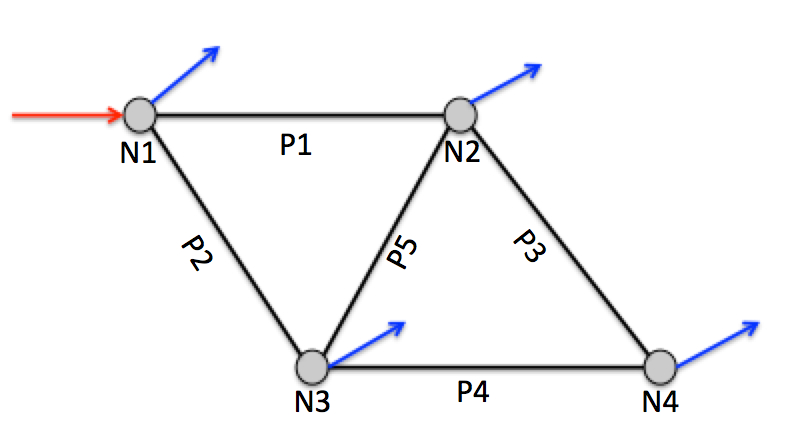
\includegraphics[width=3in]{NetworkLayout.jpg}
   \caption{Layout of Simple Network}
   \label{fig:NetworkLayout} 
\end{figure}

% Requires the booktabs if the memoir class is not being used
\begin{table}[htbp]
   \centering
   \caption{Node and Pipe Data}
    \begin{tabular}{p{1in} p{1in} p{1in} p{1in} } % Column formatting, @{} suppresses leading/trailing space
    \hline
    \hline
Pipe ID & Diameter (inches) & Length (feet) & Material \\
\hline
P1 & 8 & 800 & PVC  \\
P2 & 8 & 700 & PVC  \\
P3 & 8 & 700 & PVC  \\
P4 & 8 & 800 & PVC  \\
P5 & 6 & 600 & PVC  \\
\hline
\hline
Node ID & Demand (CFS) & Elevation (feet) & ~~ \\
\hline
N1 & 2.0 & 0.0 & ~~ \\
N2 & 4.0 & 0.0 & ~~ \\
N3 & 3.0 & 0.0 & ~~ \\
N4 & 1.0 & 0.0 & ~~ \\
   \end{tabular}
   \label{tab:PipeData}
\end{table}
\clearpage

Build an EPANET model, using the Hazen-Williams head loss model of the network.  From your model preparations and/or the actual simulation runs:

\begin{enumerate}[a)]
\item Write the node equations of continuity for Nodes 1-4. Use the naming convention on the figure.
\item Write the head loss equations for each of the pipes in the system, use the naming convention on the figure.
\item  Make a screen capture of the EPANET program showing your network map, with the Node ID and Node Pressures displayed on the map, and with the Pipe ID and Pipe Flow Rates on the map.
\item Determine the flow rate in each pipe of the network, for the case where the total head at Node 1 is 100 feet.\footnote{You can add a reservoir to Pipe 0 (the red link in the drawing), and adjust total head in that reservoir until computed head at Node 1 is 100 ft.  The connecting Pipe 0 parameters are pretty arbitrary.  Use a short, fat, smooth pipe in such instances, so there is virtually no head loss between the fictitious reservoir and the network.}
%\item Determine the Darcy-Weisbach friction factor in each pipe of the network.\footnote{The program will report this value for each pipe, even if you are using Hazen-Williams head loss model}
\item Make a table that lists each node name, node elevation, and the resultant pressure in U.S. Customary units.
\item Make a table that lists each pipe name, length, diameter, Hazen-Williams coefficient, and the resultant flow rate in U.S. Customary units.
\item Using the simulation results, determine the head loss from Node 1 to Node 4.
%\item Determine the head at Node 4
\item Identify the node with the lowest pressure in your solution.
%\item Compare the head loss from Nodes 1 to 4 determined by EPANET and the by-hand solution in the prior problem.
\end{enumerate}

%Submit the above items as content in a technical memorandum that includes a description of how the model was built and a discussion and interpretation of the results.

Attach the EPANET output report to your solution.
\clearpage


\end{enumerate}

\end{document}  

%%%%%%%%%%%%%%%%%%%%%%%%%%%%%%%%%%%%%%%%%%%%%%%%%%%%%%%
%%%%%%%%%%%%%%% PROBLEM 2 %%%%%%%%%%%%%%%%%%%%%%%%%%%%

\item Figure \ref{fig:primary-network} is a layout of a water distribution system for the SomewhereUSA subdivision. 
The blue line segments are pipes (ductile iron) and are labeled (P1, P2, . . . ). The blue circles are nodes and are labeled (N1, N2, . . . ).  The yellow polygons represent the demand lots assigned to each node. For example, node N2 supplies the six (6) individual lots located near the node.

\begin{figure}[h!] %  figure placement: here, top, bottom, or page
   \centering
   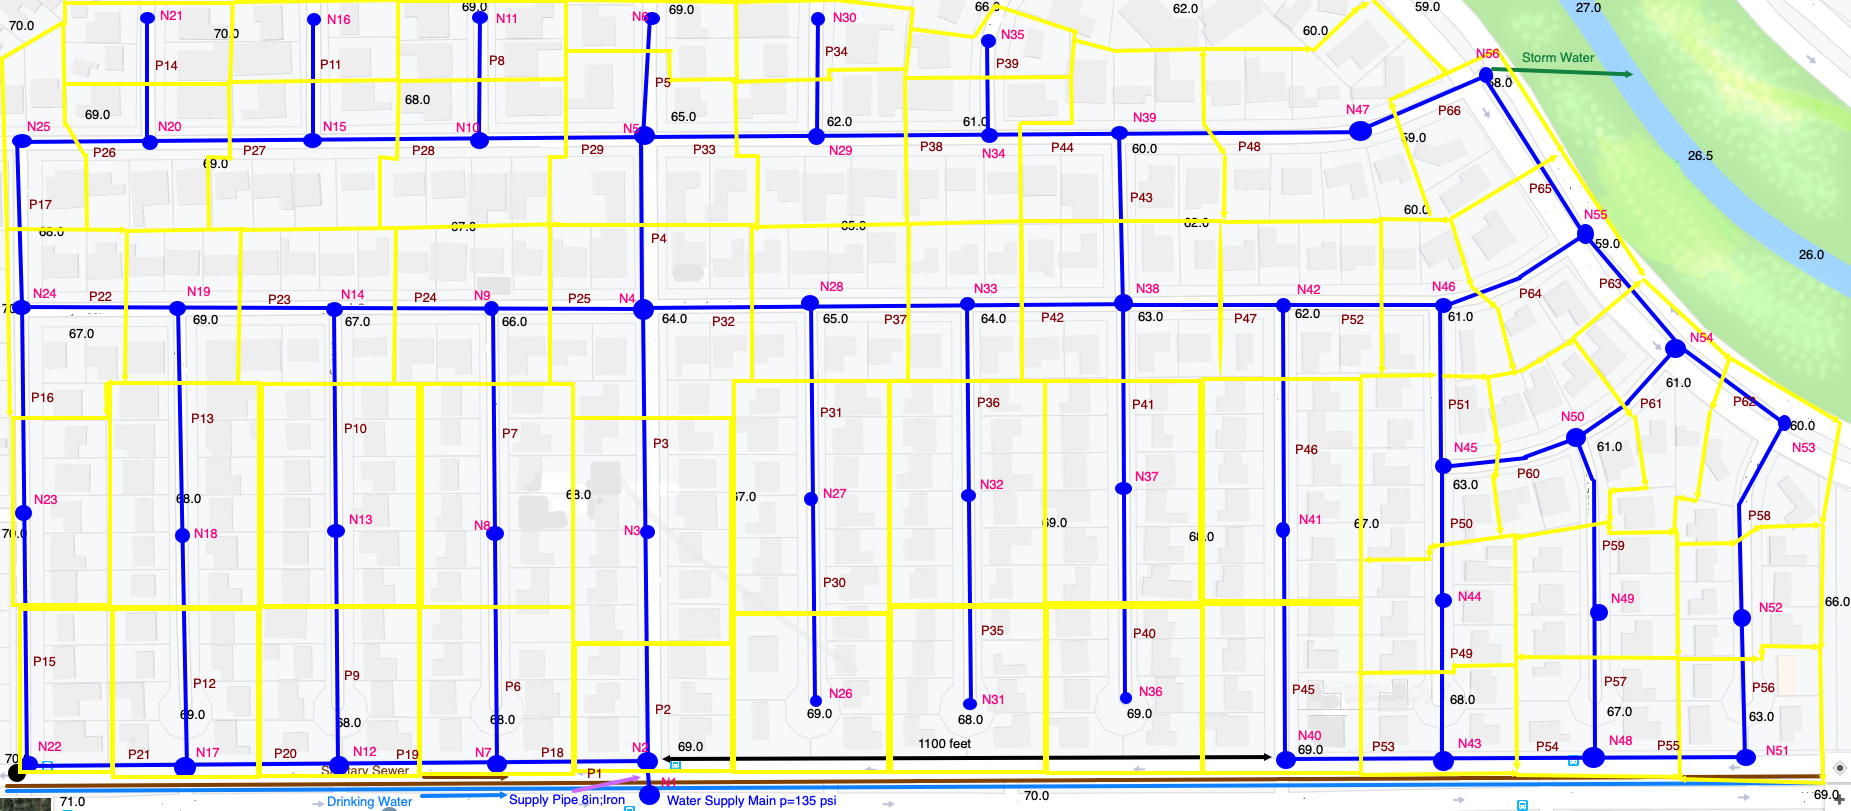
\includegraphics[width=6.5in]{SomewhereClipNodes.png} 
   \caption{Somewhere USA Water Distribution (Skeleton) System}
   \label{fig:primary-network}
\end{figure}

The distribution system is connected to the supply main at node N1. 
This large water main supplies water at 135 psi. pressure. 
The pipe connecting node N1 to N2 is an 8-inch diameter, ductile iron pipe. The remaining pipes are 2-inch diameter, ductile iron pipe.

The system is to be modeled using the United States Environmental Protection Agency, EPANET  hydraulic and water quality simulator. Use RG-195 and the San Marcos Texas manual for statutory requirements as necessary:

\begin{enumerate}[1)]
\item Using the naming convention in the drawings, determine the individual pipe lengths and produce a table of pipe length, and diameter by pipe ID. Include this table in your solution report;
\item Produce a land surface elevation map; include the map in your solution report (you did this in an earlier exercise, you can reuse your map and need not create a new one;
\item Using the naming convention in the drawings, determine the individual node elevations (offset as necessary to ensure the pipe network is buried a sufficient depth throughout the subdivision) and produce a table of node elevation by node ID;
\item Determine magnitude and location of minimum pressure in the system at average demand (reuse your earlier exercise solutions);
\item Determine magnitude and location of minimum pressure in the system at peak demand;
\item Determine magnitude and location of maximum pressure in the system at average demand;
\item Determine magnitude and location of maximum pressure in the system at peak demand;
\item Determine if there are low-pressure portions of the system that need to be mitigated by changing pipe diameters, if so, adjust the diameters and present the adjusted design as a second, independent simulation;
\item Apply a demand pattern multiplier and simulate time-varying behavior in the distribution system;
\end{enumerate}